\section*{Zielsetzung}
Das Ziel dieses Versuchs ist es, die Fallensteifigkeit einer optischen Pinzette zu bestimmen und mit dieser Kräfte und Geschwindigkeiten von Vesikeln in einer Zwiebelzelle zu untersuchen.
Außerdem soll mit Hilfe der Fallensteifigkeit und des Äquipartitionstheorems die Boltzmannkonstante bestimmt werden.
Der Transport von Vesikeln mittels Myosin-Motoren dient dabei als praktisches Beispiel für eine Anwendung in einem biophysikalischen System.

\section{Theorie}
In diesem Abschnitt wird zunächst das grundlegende Funktionsprinzip einer optischen Falle erläutert.
Anschließend wird der Zusammenhäng zwischen Fallensteifigkeit und Boltzmannkonstante durch das Äquipartitionstheorem beschrieben, um
weiter auf die Spektrale Leistungsverteilungsfunktion und auf den Einfluss der absoluten axialen Position einzugehen.
Abschließend wird der Transport von Vesikeln innerhalb von Zellen durch Myosin-Motoren beschrieben.
\subsection{Optische Falle}
Da Photonen einen Impuls tragen, können sie auch eine Kraft auf andere Objekte ausüben.
Die Größenordnung dieses Effekts legt nahe, die Kräfte auf Atome, Moleküle oder kleine biologische Organismen zu untersuchen.
Bei einer optischen Falle wird ein Laser von unten auf ein dielektrisches Material fokussiert, sodass ein Impulsübertrag durch 
Brechung und Streuung am Material (hier zum Beispiel ein mikrometer großes Quarzkügelchen) möglich wird.
Die Streuung bewirkt einen Kraftübertrag in Lichtausbreitungsrichtung, 
während die Brechung eine entgegengesetzte Gradientenkraft erzeugt. 
Sind diese Kräfte ausgeglichen ist das Objekt in der Falle gefangen 
und befindet sich in einem stabilen Gleichgewicht. Die Kräftewirkung bei kleiner Auslenkung
aus dieser Gleichgewichtslage ist in Abbildung \ref{fig:Kräfte} dargestellt.




\begin{figure}[H]
    \centering\captionsetup{format=plain}
    \includegraphics[width=0.8\textwidth]{Bilder/OP_Kräfte.png}
    \caption{Schematische kräftewirkung bei einer kleinen Auslenkung des eingefangenen Objekts aus der Gleichgewichtsposition  \cite{ref10}. Links ist der Fall einer Auslenkung weg vom Zentrum zu sehen, die resultierende Kraft wirkt wieder zurück zum Zentrum. Auf der rechten Seite ist das Objekt lediglich vertikal nach oben verschoben, sodass die resultierende Kraft nach unten wirkt.}
    \label{fig:Kräfte}
\end{figure}

Wichtig bei diesem Modell ist, dass die Wellenlänge des Laserlichts
deutlich kleiner als das untersuchte Objekt ist, damit die Strahlenoptik 
noch gültig ist. Im Vorliegenden Versuch ist diese Bedingung bei allen Aufgabenteilen erfüllt. 

\subsection{Äquipartitionstheorem}
Das Äquipartitionstheorem besagt, dass ein Teilchen im thermischen Gleichgewicht 
eine Energie von $E=\frac{1}{2}k_B T$ pro Freiheitsgrad besitzt. Dabei bezeichnet $T$ die Temperatur des gesammten Systems und $k_B$ die 
Boltzmannkonstante, die die Teilchenzahl eines idealen Gases mit der gesamten kinetischen Energie über die ideale Gasgleichung in Verbindung setzt.
Die Energie eines einzelnen Teilchens im harmonischen Potential beträgt außerdem $E=\frac{1}{2}k x^2$. $x$ bezeichnet hier die Auslenkung eines Teilchens aus der
Ruhelage und $k$ die Federkonstante. Im Falle einer optischen Falle wird die Federkonstante auch Fallensteifigkeit genannt und die 
Auslenkung kommt durch die zufällige Brownsche Bewegung zustande. Somit ist hier lediglich die statistische Varianz $<\!\!x^2\!\!>$ in der Position eines Teilchens relevant.
Durch Gleichsetzen ergibt sich somit für ein eingefangenes Teilchen im thermischen Gleichgewicht eine mittlere Energie von
\begin{equation}
    \frac{1}{2}k <\!\!x^2\!\!> = \frac{1}{2}k_B T.
\end{equation}
\subsection{Spektrale Leistungsverteilungsfunktion}
Die Brownsche Bewegungstheorie gibt 
Aufschluss über das Spektrum der Varianz in der Position eines Teilchens,
welche durch zufällige Bewegungsänderungen entstehen.
Es wird ein Teilchensystem betrachtet, in dem die Stöße der Teilchen durch eine zufällige
Kraft $F(t)$ modelliert werden. Es wird für ein Teilchengas im thermischen Gleichgewicht erwartet, 
dass die Stöße unkorreliert sind. Sind die Korrelationszeiten sehr 
klein, ergibt sich für die Verteilung der
Kraft ein ”weißes Rauschen”. Bei einer stark gedämpften
Teilchenbewegung führt dies auf die Bewegungsgleichung
\begin{equation}
    \beta \dot{x}(t) + k x(t) = F(t).
\end{equation}


Dabei bezeichnet $\beta$ den hydrodynamischen Zugwiderstandswert $\beta = 3 \pi \eta d$
mit der Viskosität $\eta$ und dem Teilchendurchmesser $d$.

Das Leistungsspektrum der Bewegung ergibt sich über das
Wiener-Khinchin-Theorem mittels einer Fouriertransfomation der zeitlich gemittelten Autokorrelationsfunktion zu
\begin{equation}
    S_{xx}(f)=\sqrt{\frac{k_B T}{\pi^2 \beta (f^2+f_0^2)}}.
\end{equation}

Hierbei ist $f_0 = \frac{k}{2 \pi \beta}$ die Roll-Off-, oder auch Dämpfungsfrequenz .
\subsection{Einfluss der absoluten axialen Position}
Da der hydrodynamische Zugwiderstandswert $\beta$ nichtlinear von der Höhe 
eines Teilchens oberhalb der Oberfläche (zum Beispiel der Probenkammer) abhängt, 
ist die absolute axiale Position eines Teilchens in der optischen Falle ein wichtiger experimenteller Parameter.
Gleichzeitig wirkt der Effekt der fokalen Verschiebung: durch die unterschiedlichen Brechungsindizes an der Kammergrenzschicht verschiebt sich die Fokussierung des Lasers.
Beim Versuch soll der Einfluss der axialen Position auf das Detektorsummensignal untersucht werden (siehe Abbildung \ref{fig:fokal}).

\begin{figure}[H]
    \centering\captionsetup{format=plain}
    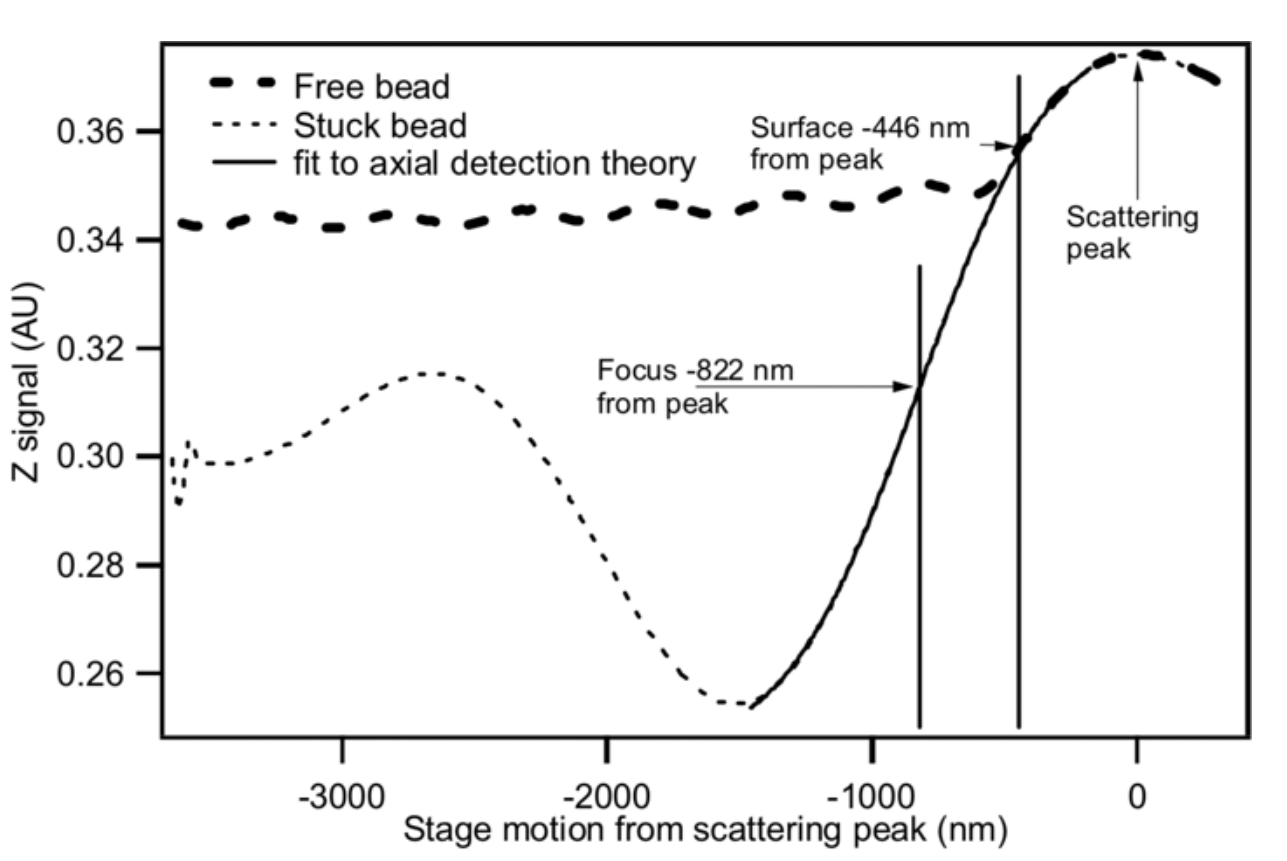
\includegraphics[width=0.7\textwidth]{Bilder/OP_Fokal.png}
    \caption{Das Detektorsummensignal als Funktion der axialen Position für ein festes und ein freies eingefangenes Kügelchen  \cite{anleitung}. Der Fit wird durch Gleichung \ref{eq:A1} beschrieben.}
    \label{fig:fokal}
\end{figure}
Die Intensitätsverteilung in der rückseitigen Brennebene des Kondensor-Objektivs 
wird moduliert, wenn sich das Kügelchen durch den Fokus des Lasers bewegt.
Der Bereich zwischen den
Extremalpunkten der festen-Kügelchen-Kurve wird durch die Gleichung

\begin{equation}
    \frac{I_z}{I}(z)\propto \Bigl( 1 + \Bigl(\frac{z}{z_0}\Bigr)^2 \Bigr)^{\frac{1}{2}}\sin\Bigl(\tan^{-1}\Bigl(\frac{z}{z_0}\Bigr)\Bigr)
    \label{eq:A1}
\end{equation}
beschrieben. Dabei bezeichnet $z$ die axiale Auslenkung von der Strahltaille
und $z_0=\frac{\pi w_0^2}{\lambda}$ die Rayleighlänge des Brennpunktes mit der Strahltaille $w_0$ und der Wellenlänge $\lambda$.
\subsection{Transport von Vesikeln in einer Zwiebelzelle}
Die bei der optischen Pinzette beobachtbaren Kräfte liegen in der Größenordnung von Mikro- und Nanonewton.
Damit eignet sich diese Methode besonders für Untersuchungen in der Mikrobiologie, zum Beispiel um die Kräfte und Geschwindigkeiten zu vermessen,
die beim Transport von Stoffen innerhalb einer Zelle auftreten.
Um Nahrung, Müll, Informationen und einiges mehr zu transportieren,
werden diese in Membran-gebundenen Vesikeln durch Myosin-Motoren entlang von Aktin-Mikrofasern bewegt.
Myosin ist ein Motorprotein, welches an der Faser aus Aktin Strukturproteinen zieht und sich entlang dieser krümmen kann.
Somit ist es möglich die Vesikel entlang einer solchen Spur weiterzureichen.
